\documentclass{article}
\usepackage[utf8]{inputenc}
\usepackage{graphicx}
\usepackage{listings}
\usepackage{subcaption}
\usepackage{amsmath}
\usepackage{mathtools}
\usepackage{geometry}
\usepackage{float}
 \geometry{
 a4paper,
 total={175mm,257mm},
 left=20mm,
 top=20mm,
 }
\title{Homework-4}
\author{Susan Sapkota and Anish A. Adhikari}
\date{November 2020}

\begin{document}

\maketitle
\section{Introduction}
Scientific problem usually involves functions of various parameter in equations(like Maxwell equation,Wave equation). Such equations are in partial differential form which cannot be solved analytically due complexity. Most of the real life problem involving partial differential equation needs multiple differentiation and integration in curvilinear domain can be solved using numerical method.

 In this homework, we compute derivatives, integrals and error in such calculation on smooth rectangular domain denoted my $\Omega$. The main idea is to use one to one smooth mapping $(x,y)=(x(r,s),y(r,s))$ from a reference element $\Omega_R=(r,s)\in [-1,1]^2$ to $\Omega$. One can technically transfer the computation like differentiation and integral from $\Omega$ to $\Omega_R$.
\section{Methods}
\subsection{Differentiation on $\Omega$}
Let $u=u(x,y)$ be a continuously differentiable function of x and y, where $(x,y) \in \Omega$. Let us approximate the partial derivative of u with respect to x and y. Firstly, consider $x=x(r,s)$ and $y=y(r,s)$ as functions of r and s where $(r,s) \in \Omega_R = [-1,1]^2$. Then apply chain rule which gives
\begin{equation}
    \dfrac{\partial u}{\partial x}
        = \dfrac{\partial r}{\partial x} \dfrac{\partial u}{\partial r}
        + \dfrac{\partial s}{\partial x} \dfrac{\partial u}{\partial s} \\[4mm]
\end{equation}
\begin{equation}
    \dfrac{\partial u}{\partial y}
        = \dfrac{\partial r}{\partial y} \dfrac{\partial u}{\partial r}
        + \dfrac{\partial s}{\partial y} \dfrac{\partial u}{\partial s} \\[4mm]
\end{equation}

We introduce a Cartesian grid on the reference element $\Omega_R = [-1,1]\times [-1,1]$. Let nr and ns be the number of grid size in r and s direction respectively. We discretized the grid with step size given by $hr=\dfrac{2}{nr}$ and $hs=\dfrac{2}{ns}$ respectively. Then we can define ith position of the grid by,
\begin{align*}
   &  r(i) = -1 + i \times hr\\
    & s(i) = -1 + i \times hs\\
\end{align*}
We computed $u_r = \dfrac{\partial u}{\partial r}$ and $u_s = \dfrac{\partial u}{\partial s}$ using standard finite difference formula describe in section 2.3. We need to find $r_x$, $r_y$, $s_x$ and $s_y$ to apply equation 1 and 2 to compute $u_x$ and $u_y$. We computed $x_r$, $y_r$, $x_s$ and $y_s$ using standard finite difference formula describe in section 2.3. Let us take u=x in equation 1 and u=y in equation 2 then we get, 
\begin{equation*}
    \begin{bmatrix}
    r_x & s_x \\
    r_y & s_y \\ 
    \end{bmatrix} 
     \begin{bmatrix}
    x_r & y_r \\
    x_s & y_s \\ 
    \end{bmatrix} 
    = 
    \begin{bmatrix}
        1 & 0 \\
        0 & 1 \\
    \end{bmatrix}
\end{equation*}
Let us consider $2^{nd}$ matrix on left side is invertible(Determinant is non-zero). Then we multiply by inverse of matrix to get 
\begin{equation}
       \begin{bmatrix}
    r_x & s_x \\
    r_y & s_y \\ 
    \end{bmatrix}
    =
     {\begin{bmatrix}
    x_r & y_r \\
    x_s & y_s \\ 
    \end{bmatrix}}^{-1}
    = 
   \frac{1}{J(r,s)} \times
     \begin{bmatrix}
    y_s & -y_r \\
    -x_s & x_r \\ 
    \end{bmatrix} 
\end{equation}
where $J(r,s) = x_ry_s - x_sy_r $

\subsection{Integration on $\Omega$}
 We computed integrals on rectangular domains given by
\begin{equation}
    \int_\Omega f(x, y) \, dx dy
        = \int_{-1}^1 \int_{-1}^1 f(x(r, s), y(r, s)) \, J(r, s) \, dr ds 
\end{equation}
where $J(r,s) = x_ry_s - x_sy_r $ is the surface element. We approximated second integrand by using 2D trapezoidal rule described in section 2.4.

\subsection{Finite Difference}
We use three-point stencil of a point in the grid i.e stencil with point itself with its two neighbor to write finite difference approximation to derivatives at grid point.Let $x \in [a,b]$ and $x_i=a+i\times h$ and i=0,1,2,.....,n. Let spacing between points in grid be $h=\frac{b-a}{n}$ then three-point stencil of point x in grid is given by ${x-h,x,x+h}$. From Taylor series, we have 
\begin{enumerate}
    \item $f(x+h) = f(x)+hf'(x)+\frac{h^2}{2}f"(x)+\frac{h^3}{6}f"'(x)+\frac{h^4}{24}f""(x)+O(h^5)$
  \item $f(x-h) = f(x)-hf'(x)+\frac{h^2}{2}f"(x)-\frac{h^3}{6}f"'(x)+\frac{h^4}{24}f""(x)+O(h^5)$
\end{enumerate}
We can subtract 1 and 2 to get 
\begin{equation}
    f'(x) \approx \frac{f(x+h)-f(x-h)}{2h} + O(h^2)
\end{equation}

In our case, $x\in [-1,1]$ and consider equidistant grid $x_i=-1+i\times h$ and i=0,1,2,3,.....,n with $h=\frac{2}{n}$. By manipulating above Taylor series expansion, we approximate $f^{'}(x_i)$ given using biased stencil i.e. in the interior we used centred stencil (eqution-5), left and right with biased stencil given by,
\begin{enumerate}
    \item $f^{'}(x_i)= \frac{-1.5f(x_i)+2f(x_{i+1})-0.5f(x_{i+2})}{h},  i=0$
    \item $f^{'}(x_i)=\frac{0.5f(x_{i+1})-0.5f(x_{i-1})}{h},  i=1,......,n-1$
    \item $f^{'}(x_i) = \frac{1.5f(x_i)-2f(x_{i-1})+0.5f(x_{i-2})}{h},  i=n$
\end{enumerate}
The error is order of $O(h^2)$.
\subsection{2D Trapezoidal Rule }
Let us consider double integrals given by, 
\begin{equation}
    I = \iint_\Omega f(x,y) dxdy,
\end{equation}
where $\Omega$ is a domain given by 
\begin{equation*}
    \Omega = {(x,y) \in ( x \in [a,b], y \in [c,d])}
\end{equation*}
one can write integral in iterated form as, 
\begin{equation*}
I = \int_{a}^b \left ( \int_{c}^d f(x,y) dy \right ) dx
\end{equation*}
Numerically we can compute inner integral by one dimensional quadrature rule by keeping x as constant. The values obtained are then used to approximate the outer integral by 1D trapezoidal rule. To be more precise, we consider as 
\begin{enumerate}
     \item $F(x)=\int_c^{d} f(x,y)dy$
     
    \item  $I = \int_a^{b} F(x)dx$
\end{enumerate}
Then we approximate I with 1D trapezoidal rule. Let us discretize [a,b] into n equally space panel with stepsize as 
$h=\frac{b-a}{n}$ and $x_j = a+j\times h$ and j=0,1,2,.....,n. I is approximated by, 
\begin{equation*}
    I \approx T_{n+1}(F) = h \left( \frac{1}{2} F(x_0) + F(x_1)+F(x_2)+.........+ F(x_{n-1})+\frac{1}{2}F(x_n) \right)
\end{equation*}
with $Error_n(F)= \int_a^{b}F(x)dx-T_{n+1}(F)=-\frac{h^2(b-a)}{12} f^{"}(c_n)=O(h^2)$ for some $c_n$ in the interval [a,b].
We approximate again to compute $F(x_j)$. let us discretize again [c,d] into $n_j$ equally spaced panel with $h_j = \frac{d-c}{n_j}$ and $y_{j,k}=c+k\times h_j$ and k=0,1,2,....,n. Then $F(x_j)$ is approximated as
\begin{equation*}
    F(x_j)=\int_c^{d}f(x_j,y)dy \approx h_j \left ( \frac{1}{2}f(x_j,y_{j,o})+f(x_j, y_{j,1})+.......+f(x_j, y_{j,n_{j-1}}) + \frac{1}{2} f(x_j,y_{j,n_j}) \right)
\end{equation*}
We can say that order of accuracy is two and total error is given by,
\begin{equation*}
    Error_{total} = O(h^2+max_j h_j^2)
\end{equation*}
\subsection{Laplace} 
We already have partial of u with respect  to x and y given by equation 1 and 2 and computed using finite difference formula described in section 2.3. Now again, we use finite difference of section 2.3 to computed derivative of $u_x$ and $u_y$ in the r-direction and s-direction giving out $u_{xr}$,$u_{xs}$,$u_{yr}$,$u_{ys}$. The lapacian is 
\begin{align}
   & u_{xx}=r_x u_{xr}+r_s u_{xs}
   & u_{yy}=r_y u_{yr}+r_s u_{ys}
   \end{align}
\subsection{Error}
We computed $u_x$ and $u_y$ for function $u(x,y)$  and $(x,y)=(x(r,s),y(r,x))$ using process describe in section 2.1. we calculated $(u_{exact})_x$ and $(u_{exact})_y$ using simple mathematical partial differentiation for given $u(x,y)$.The error formula in integration (equation4) is given by,
\begin{align}
    & \text{err}(h_r, h_s)
        = \left|
            \int_{\Omega}
                \left(
                    u_x(x, y) + u_y(x, y) -
                        \big[
                            (u_\text{exact})_x(x, y) + (u_\text{exact})_y(x, y)
                        \big]
                \right)^2
                \, dx dy \right|^{\tfrac{1}{2}} 
\end{align}
        where $h_r$ and $h_s$ are the step sizes. We computed above integral using 2D Trapezoidal Rule described in section 2.3. The effective grid-size $h_{eff}=\sqrt{h_r h_s maxJ}$.

We used equation-7 and 2D trapezoidal rule to compute error in integration of laplacian  given by, 
\begin{align}
    & \text{err}(h_r, h_s)
        = \left|
            \int_{\Omega}
                \left(
                    u_{xx}(x, y) + u_{yy}(x, y) -
                        \big[
                            (u_\text{exact})_{xx}(x, y) + (u_\text{exact})_{yy}(x, y)
                        \big]
                \right)^2
                \, dx dy \right|^{\tfrac{1}{2}} 
\end{align}
where $(u_{exact})_{xx}$ and $(u_{exact})_{yy}$ is calculated using simple theoretical partial differentiation for given $u(x,y)$.

\section{Result and Discussion}
We used $n_s=n_r=35$ for plotting grid and $n_s=n_r=(5,35,75,90,95)$ for plotting error in integral and laplacian.

We used the simple case for testing in which we can easily calculate integral by analytically. for example, for the case of $x = r\cos(s),
y = r\sin(s)$, we know what to expect for a curvilinear grid (two cones
with rounded bases, because our angle, $s$, varies from $-1$ to $1$ and so
does our radius, $r$). The grid size is given in figure-1 which is symmetrical on axis.

$x = r\cos(s) \quad y = r\sin(s) \quad u = 1$.
\begin{align*}
    & \int_\Omega u(x, y) \, dx dy = \int_{-1}^1 \int_{-1}^1 J \, dr ds \\
    & J = \begin{vmatrix} x_r & x_s \\ y_r & y_s \end{vmatrix}
        = \left| \begin{array}{rr}
            \cos(s) & -r\sin(s) \\
            \sin(s) & r \cos(s)
        \end{array} \right|
        = r \left( \cos^2(s) + \sin^2(s) \right) = r \\
    & \int_{-1}^1 \int_{-1}^1 \, J \, dr ds
        = \int_{-1}^1 \int_{-1}^1 r \, dr ds
        = 0 \quad \text{(by symmetry)}
\end{align*}
\begin{figure}[h]
\centerline{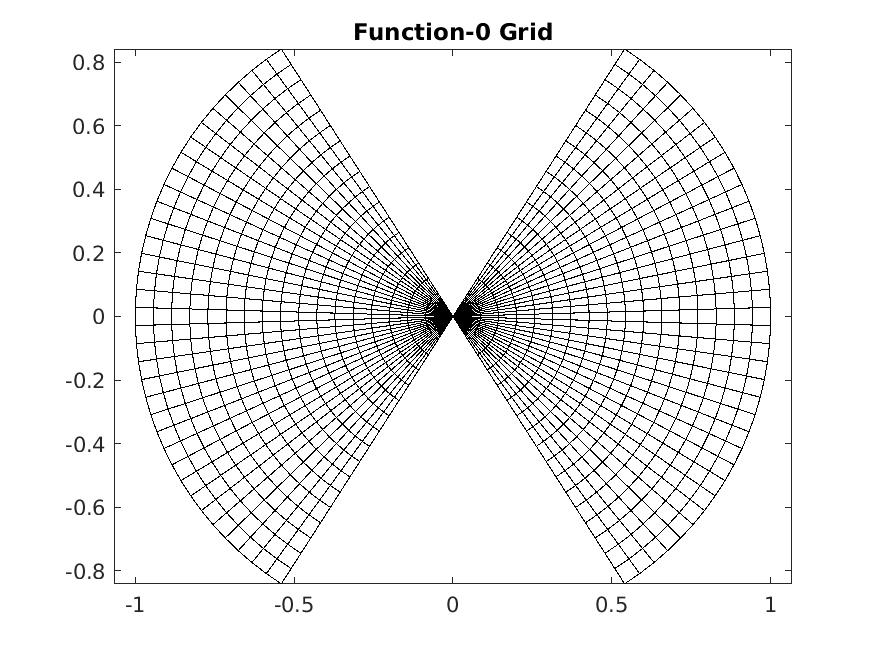
\includegraphics[scale=.5,width=1.0\linewidth,height=0.5\textheight]{grid_0.jpeg}}

\caption{Function-0 with x=rcos(s), y=rsin(s) and u(x,y)=1 }
\label{fig}
\end{figure}
We got 0 for all except for 75 is $5.56e-20$ which is almost zero. So, our approximation result for integral matches with the theoretical value.

$x = r + 0.1 s$,$y = s$,$u = sin(x)cos(y)$ is combination-1. we find theoretical derivative of u in direction of x any y as $(u_{exact})_x = cos(x)cos(y)$ and $(u_{exact})_y = -sin(x)sin(y)$. we plot log-log graph of error in integration vs effective grid size in figure 2(b).The error in integration is similar to $O(h^2)$ line  as expected from theory since we used central difference to compute derivative (section-2.3) and trapezoidal rule (section-2.4) for the error computation. similarly, we did compute laplacian and integrate to compute to compute error.we did plot log-log plot of integration of laplacian vs effective grid size in figure 2(c). The error line is almost parallel towards the top however it  doesn't look parallel at bottom. We thought reason might be due to accumulation of error in twice differentiation and max norm used in error formula.

We used $x=(2+r+0.1 sin(5\pi s))cos(0.5\pi s)$,$x=(2+r+0.1 sin(5\pi s))sin(0.5\pi s)$, $u(x,y)= e^{x+y}$ for combination-2. The partial differentiation in direction of x and y for the function u are $(u_{exact})_x=e^{x+y}$ and $(u_{exact})_y=e^{x+y}$. The grid is shown in figure 3(a). The log-log plot of error in integration and effective grid size is almost parallel to $O(h^2)$ as expected from theory. The irregularity might be due to max norm. similarly, For the error in laplacian, the exact differentiation in direction of x and y are $(u_{exact})_{xx}=e^{x+y}$ and $(u_{exact})_{yy}=e^{x+y}$.The log-log plot for the laplacian integration looks parallel to $O(h^2)$ with kink in middle which might due to accumulation of error in differentiation two time and max norm.

$x=r$, $y=s+sr^2$ and $u(x,y)=x^2+y^2$ is the combination-3. The partial differentiation in direction of x and y for the function u are $(u_{exact})_x=2x$ and $(u_{exact})_y=2y$. The grid is shown in figure 3(b). The log-log plot of error in integration vs effective grid size is in figure 3(b). The error line looks parallel to $O(h^2)$. On increasing the effective grid sized, the error plot little deviate which might be due max norm that we used in calculation. We do compute laplacian for the function which are $(u_{exact})_{xx}=2$ and $(u_{exact})_{yy}=2$. The log-log plot of error in integration vs effective grid size is parallel in lower but not on the upper part might be due to max norm and error accumulation of error in twice differentiation.
In conclusion, The error in integration of both type is $O(h^2)$.


\begin{figure}
    \begin{subfigure}{\textwidth}
    \centering
    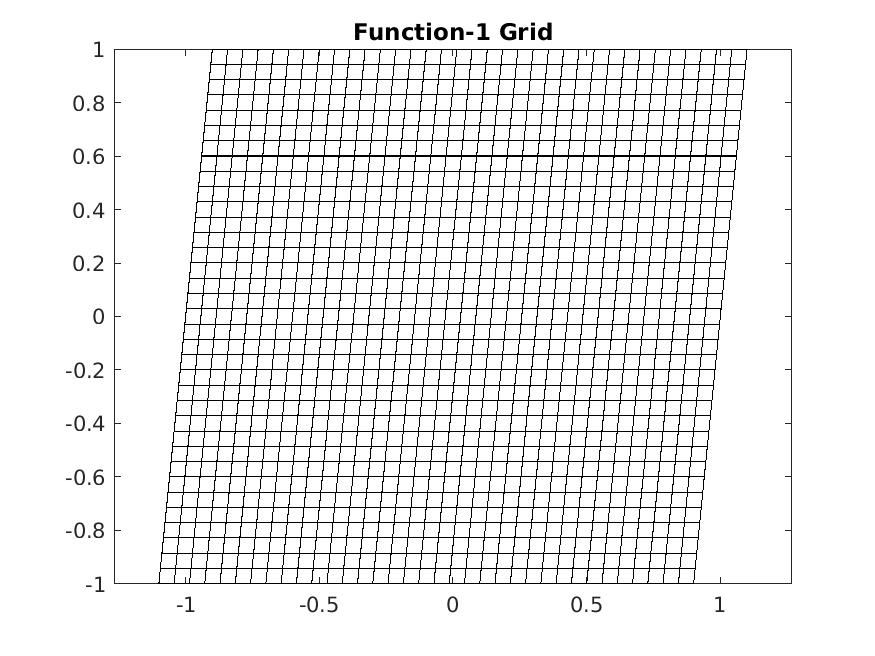
\includegraphics[scale=0.33]{grid_1.jpeg}
    \caption{Grid-1}
    \label{fig:doc1}
    \end{subfigure}

    \bigskip
    \begin{subfigure}{\textwidth}
    \centering
    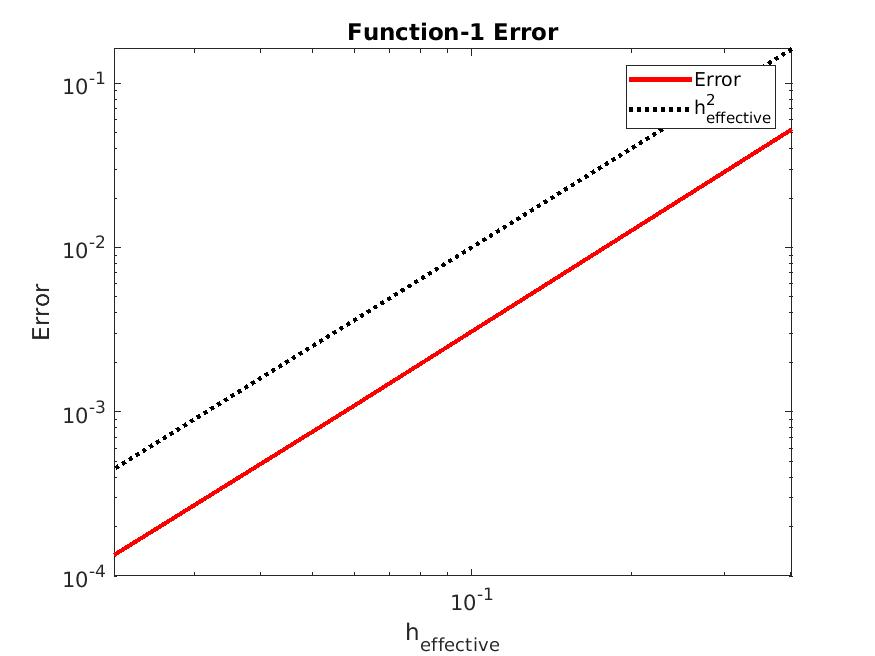
\includegraphics[scale=0.33]{error-in-1.jpg}
    \caption{Error in integration}
    \label{fig:doc2}
    \end{subfigure}

    \bigskip
    \begin{subfigure}{\textwidth}
    \centering
    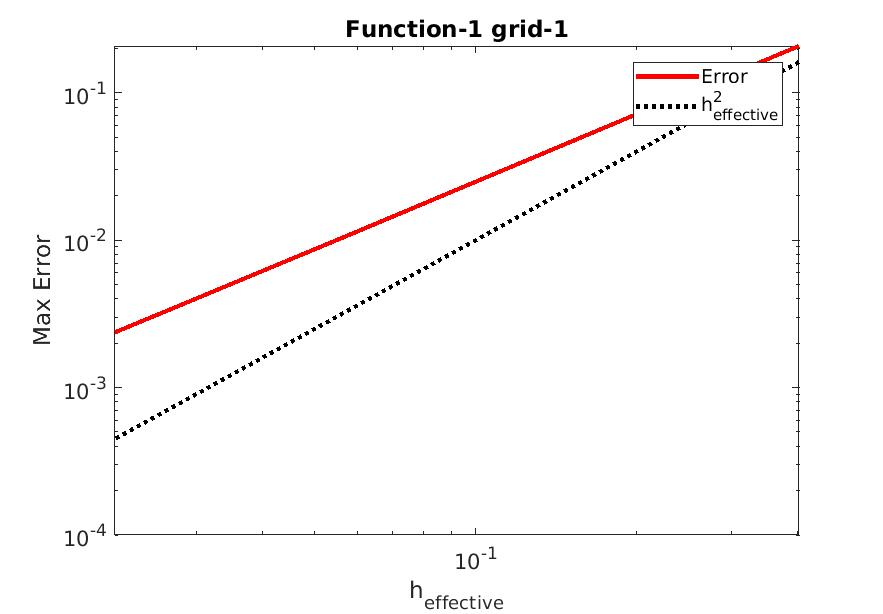
\includegraphics[scale=0.33]{error-inlaplace1.jpg}
    \caption{Error in laplace integration}
    \label{fig:doc3}
    \end{subfigure}
\caption{Combination-1:-$x = r + 0.1 s$,$y = s$,$u = sin(x)cos(y)$}
\end{figure}
\newpage 

\begin{figure}
    \begin{subfigure}{\textwidth}
    \centering
    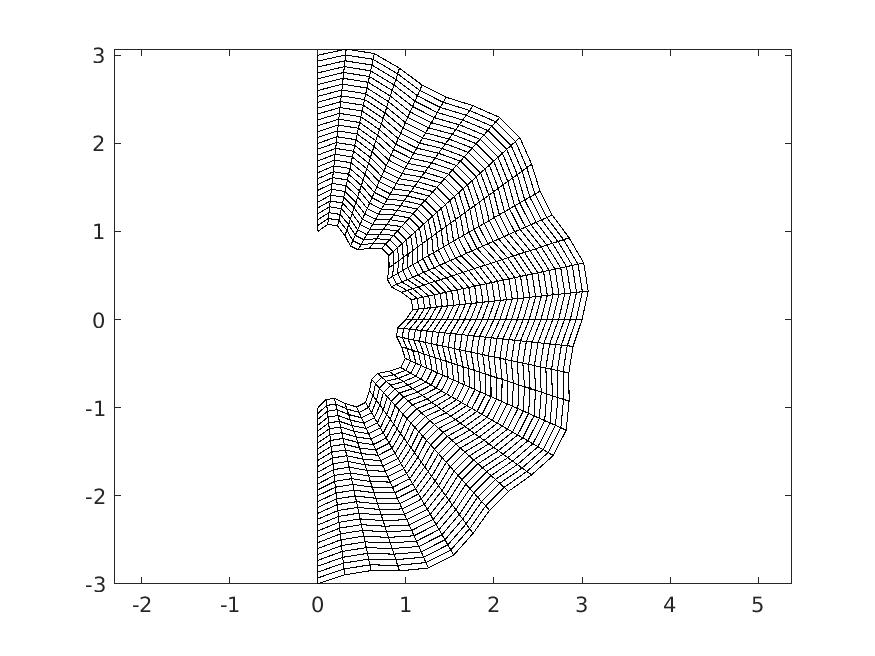
\includegraphics[scale=0.33]{grid_2.jpeg}
    \caption{Grid-2}
    \label{fig:doc1}
    \end{subfigure}

    \bigskip
    \begin{subfigure}{\textwidth}
    \centering
    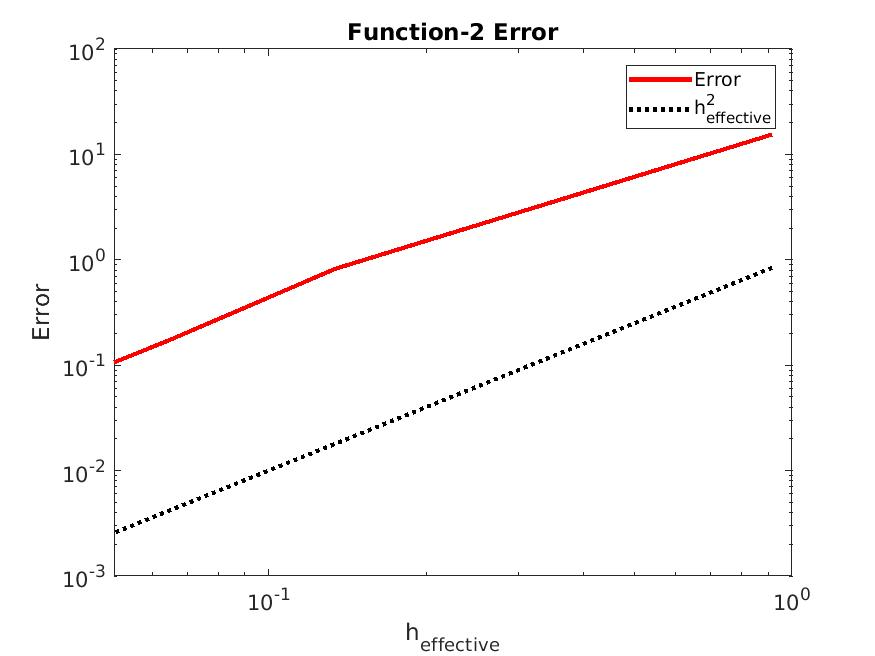
\includegraphics[scale=0.33]{error-in-2.jpg}
    \caption{Error in integration}
    \label{fig:doc2}
    \end{subfigure}
    \bigskip
    \begin{subfigure}{\textwidth}
    \centering
    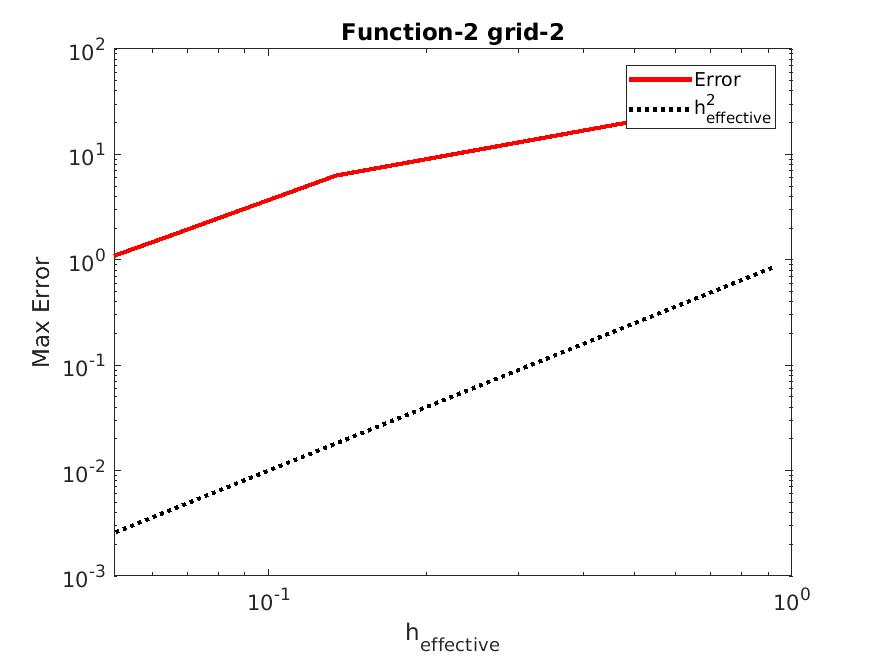
\includegraphics[scale=0.33]{error-inlaplace2.jpg}
    \caption{Error in laplace integration}
    \label{fig:doc3}
    \end{subfigure}
\caption{Combination-2:-$x=(2+r+0.1 sin(5\pi s))cos(0.5\pi s)$,$x=(2+r+0.1 sin(5\pi s))sin(0.5\pi s)$, $u(x,y)= e^{x+y}$}
\end{figure}
\newpage
\begin{figure}
    \begin{subfigure}{\textwidth}
    \centering
    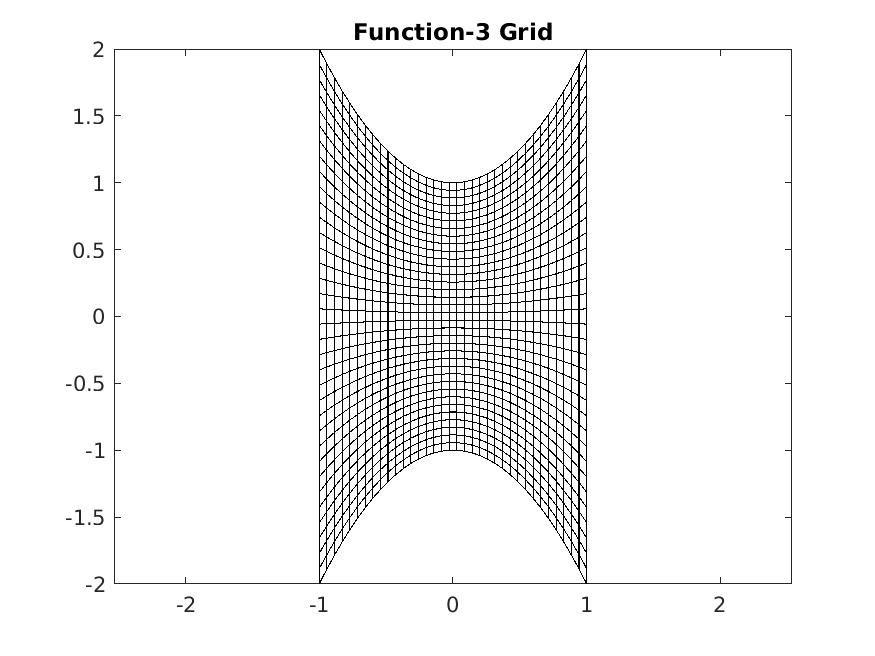
\includegraphics[scale=0.33]{grid_3.jpeg}
    \caption{Grid-2}
    \label{fig:doc1}
    \end{subfigure}

    \bigskip
    \begin{subfigure}{\textwidth}
    \centering
    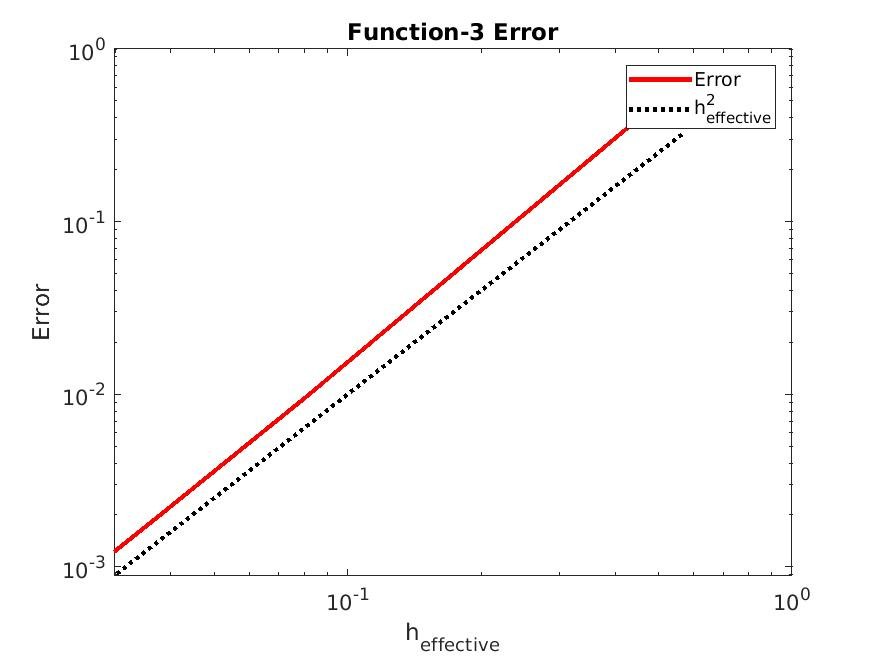
\includegraphics[scale=0.33]{error-in-3.jpg}
    \caption{Error in integration}
    \label{fig:doc2}
    \end{subfigure}
    \bigskip
    \begin{subfigure}{\textwidth}
    \centering
    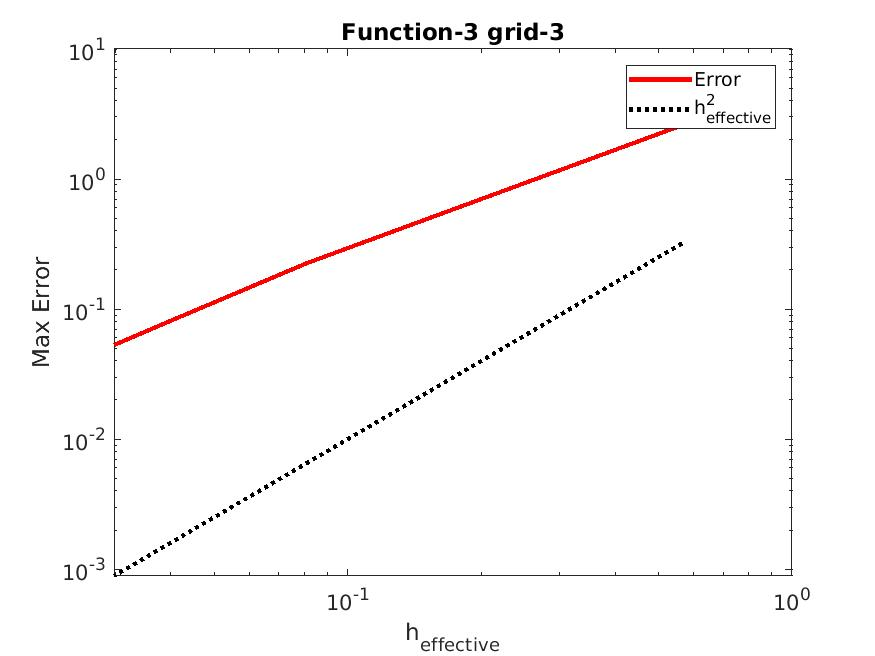
\includegraphics[scale=0.33]{error-inlaplace3.jpg}
    \caption{Error in laplace integration}
    \label{fig:doc3}
    \end{subfigure}
    
\caption{Combination-3:-$x=r$, $y=s+sr^2$ and $u(x,y)=x^2+y^2$}
\end{figure}
\newpage
 \end{document}
